\documentclass[12pt,twoside,english]{article}
\usepackage[utf8]{inputenc}

%%%%%%%%%%%%%%%%%%%%%%%%%%%%%%%%%%%%%%%%%%%%%%%%%%%%%%%%%%%%%%%%%%%%%%%
%% template for II2202 proposal
%% original 2020.08.28
%% revised  
%%%%%%%%%%%%%%%%%%%%%%%%%%%%%%%%%%%%%%%%%%%%%%%%%%%%%%%%%%%%%%%%%%%%%%%
%

%%% Local Variables:
%%% mode: latex
%%% TeX-master: "."
%%% End:

%%TC:ignore
\usepackage[paper=a4paper,dvips,top=1.5cm,left=1.5cm,right=1.5cm,
    foot=1cm,bottom=1.5cm]{geometry}


\usepackage{todonotes}          %to provide inline and margin notes
%\usepackage[T1]{fontenc}
%%\usepackage{pslatex}
\renewcommand{\rmdefault}{ptm} 
\usepackage{mathptmx}
\usepackage[scaled=.90]{helvet}
\usepackage{courier}
%
\usepackage{bookmark}

\usepackage{fancyhdr}
\pagestyle{fancy}

%%----------------------------------------------------------------------------
%%   pcap2tex stuff
%%----------------------------------------------------------------------------
 %%\usepackage[dvipsnames*,svgnames]{xcolor} %% For extended colors
 %%\usepackage{tikz}  %% Already loaded
 %%\usetikzlibrary{arrows,decorations.pathmorphing,backgrounds,fit,positioning,calc,shapes}

%% \usepackage{pgfmath}	% --math engine
%%----------------------------------------------------------------------------
%% \usepackage[latin1]{inputenc}
\usepackage[utf8]{inputenc} % inputenc allows the user to input accented characters directly from the keyboard
\usepackage[english]{babel}
%% \usepackage{rotating}		 %% For text rotating
\usepackage{array}			 %% For table wrapping
\usepackage{graphicx}	                 %% Support for images
\usepackage{float}			 %% Suppor for more flexible floating box positioning
\usepackage{color}                       %% Support for colour 
\usepackage{mdwlist}
%% \usepackage{setspace}                 %% For fine-grained control over line spacing
%% \usepackage{listings}		 %% For source code listing
%% \usepackage{bytefield}                %% For packet drawings
\usepackage{tabularx}		         %% For simple table stretching
%%\usepackage{multirow}	                 %% Support for multirow colums in tables
\usepackage{dcolumn}	                 %% Support for decimal point alignment in tables
\usepackage{url}	                 %% Support for breaking URLs
\usepackage[perpage,para,symbol]{footmisc} %% use symbols to ``number'' footnotes and reset which symbol is used first on each page
\usepackage[binary-units=true]{siunitx} %% to be able to use binary units
\newcommand{\SIadj}[2]{\SI[number-unit-product={\text{-}}]{#1}{#2}}

%% \usepackage{pygmentize}           %% required to use minted -- see python-pygments - Pygments is a Syntax Highlighting Package written in Python
%% \usepackage{minted}		     %% For source code highlighting

%% \usepackage{hyperref}		
\usepackage[all]{hypcap}	 %% Prevents an issue related to hyperref and caption linking
%% setup hyperref to use the darkblue color on links
%% \hypersetup{colorlinks,breaklinks,
%%             linkcolor=darkblue,urlcolor=darkblue,
%%             anchorcolor=darkblue,citecolor=darkblue}

%% Some definitions of used colors
\definecolor{darkblue}{rgb}{0.0,0.0,0.3} %% define a color called darkblue
\definecolor{darkred}{rgb}{0.4,0.0,0.0}
\definecolor{red}{rgb}{0.7,0.0,0.0}
\definecolor{lightgrey}{rgb}{0.8,0.8,0.8} 
\definecolor{grey}{rgb}{0.6,0.6,0.6}
\definecolor{darkgrey}{rgb}{0.4,0.4,0.4}
%% Reduce hyphenation as much as possible
\hyphenpenalty=15000 
\tolerance=1000

%% useful redefinitions to use with tables
\newcommand{\rr}{\raggedright} %% raggedright command redefinition
\newcommand{\rl}{\raggedleft} %% raggedleft command redefinition
\newcommand{\tn}{\tabularnewline} %% tabularnewline command redefinition

%% definition of new command for bytefield package
\newcommand{\colorbitbox}[3]{%
	\rlap{\bitbox{#2}{\color{#1}\rule{\width}{\height}}}%
	\bitbox{#2}{#3}}

%% command to ease switching to red color text
\newcommand{\red}{\color{red}}
%%redefinition of paragraph command to insert a breakline after it
\makeatletter
\renewcommand\paragraph{\@startsection{paragraph}{4}{\z@}%
  {-3.25ex\@plus -1ex \@minus -.2ex}%
  {1.5ex \@plus .2ex}%
  {\normalfont\normalsize\bfseries}}
\makeatother

%%redefinition of subparagraph command to insert a breakline after it
\makeatletter
\renewcommand\subparagraph{\@startsection{subparagraph}{5}{\z@}%
  {-3.25ex\@plus -1ex \@minus -.2ex}%
  {1.5ex \@plus .2ex}%
  {\normalfont\normalsize\bfseries}}
\makeatother

\setcounter{tocdepth}{3}	%% 3 depth levels in TOC
\setcounter{secnumdepth}{5}
%% Acronyms
\usepackage[acronym, nopostdot]{glossaries}
\glsdisablehyper
\makeglossaries

\renewcommand{\headrulewidth}{0pt}
%%%%%%%%%%%%%%%%%%%%%%%%%%%%%%%%%%%%%%%%%%%%%%%%%%%%%%%%%%%%%%%%%%%%
%% End of preamble
%%%%%%%%%%%%%%%%%%%%%%%%%%%%%%%%%%%%%%%%%%%%%%%%%%%%%%%%%%%%%%%%%%%%

\newacronym{AR}{AR}{augmented reality}

\title{Avoiding Multicast Acknowledgement Explosions in Multicast File Distribution Protocol}
\author{
        \textsc{Gerald Q. Maguire Jr.}
            \qquad
        \textsc{Anders Västberg}
        \mbox{}\\
        \normalsize
            \texttt{maguire}
        \textbar{}
            \texttt{vastberg}
        \normalsize
            \texttt{@kth.se}
}
\date{\today}


\lhead{II2202, Fall 2020, Period 1-2}
%% or \lhead{II2202, Fall 2020, Period 1}
\chead{Project proposal}
\rhead{\date{\today}}

\makeatletter
\let\ps@plain\ps@fancy 
\makeatother

\setlength{\headheight}{15pt}
\begin{document}

\maketitle


% \begin{abstract}
% \label{sec:abstract}

% Your abstract here.

% \end{abstract}
%%\clearpage

\selectlanguage{english}

\todo[inline]{The length of this project proposal shall not be longer than 3-5 pages (with about 400 words – 600 words describing the project) excluding title, authors, milestone chart, and appendix.

Save the document in a file with a name of the form:

author1\textunderscore{}author2-Project\textunderscore{}Plan-YYYYMMDD

Note: All sections must be descriptive and most will contain more than one sentence!
}

\section{Allocation of responsibilities}
\label{sect:alloc_responsibilities}
\todo[inline]{List authors and allocation of responsibilities. Answer the
  question: Who will be involved and what are their responsibilities within
  the project? For example, as shown above (for the authors) and below (for their responsibilities).}

Gerald Maguire is responsible for writing the test programs, writing Sections 1 and 4 (Analysis) in the report, and presenting the project plan.

Anders Västberg is responsible for collecting data using Wireshark, writing Sections 2-3, 5 in the report, and presenting the final project.


\section{Organization}
\label{sect:organization}
%\todo[inline]{One or more sentences. This describes how the project is to be organized. For example:}

The project will be organized as a two-person project, building upon previously published work and tools. 

The literature on which this project is based, primarily Jennett et al.\cite{jennett_measuring_2008}, will be used to gather data relative to participants' subjective experience, while Apple's Developer Tools will provide device-specific measures.
Once the test application is ready to be used, data collection and analysis will proceed in parallel.


\section{Background}
\label{sect:background}
\todo[inline]{Describe the background for chosen area that is going to be investigated. Write a short description of the area that is going to be investigated. It is a brief description of the necessary background knowledge of the problem area and for carrying out the project. For example:}
This project builds on the idea of multicast file distribution described in RFC1235\cite{john_ioannidis_coherent_1991}. Clients report which blocks they are missing as a vector of bits, where missing blocks are indicated by a 1 bit. The length of each block is fixed; we will assume that it is 512 bytes for this project.



\section{Problem statement}
\label{sect:problem_statement}
\todo[inline]{Describe the problem(s) that have been found in the area described in the background. Describe the problem area (in detail). For example:}

The project will investigate how to avoid so-called “acknowledgement implosion” when distributing a file using multicast. If all of the nodes that successfully receive a packet were to acknowledge it, then the sender would receive a very large number of \glspl{ACK}, when it fact it is most interested in understanding which node did not receive the packet, hence to which node (or nodes) it should retransmit the packet.

\section{Problem}
\label{sect:problem}

\todo[inline]{State a clear and concise problem that is going to be investigated.  Answer the question What is the real problem? - What is the problem or value proposition addressed by the project? – Ideally one sentence that is very concrete. For example:}

Avoiding \gls{ACK} implosion is essential to enable multicast file distribution to scale to large numbers of receivers. What techniques can we use and how should they be used.

\section{Hypothesis}
\label{sect:hypothesis}
\todo[inline]{State a hypothesis that you think would be the outcome of your investigation. Answer the question: What is your hypothesis? (Note that the hypothesis must be measurable to be confirmed or falsified. Moreover not all projects have hypothesis.).}

Avoiding \gls{ACK} implosion can be performed by sending only \glspl{NACK}, rather than sending positive \glspl{ACK}.

\section{Purpose}
\label{sect:purpose}
\todo[inline]{Explain the purpose(s) of your project / investigation (the expected deliverables from the project). Answer the question: Why do this project? (purpose/effect, i.e. – the purpose can be to save environment but the goal is to build a robot that can pick up trash.) Why would you carry out the project? For example:}

The purpose is to present one or more techniques that can be used with multicast file distribution to prevent an \gls{ACK} implosion, thus fostering the use of multicast file distribution.

\section{Goal(s)}
\label{sect:goals}
\todo[inline]{Explain the goal(s), objective(s), and/or the result(s) of your investigation. What are the expected deliverables/outcomes from the project? For example:}

An analytic model showing the advantage of using only \glspl{NACK} versus positive \glspl{ACK} will be derived based on fitting curves to the experimental data for both forms of multicast file distribution. This model can be used to invalidate the hypothesis.

\section{Tasks}
\label{sect:tasks}
%\todo[inline]{Describe the tasks and sub tasks that are necessary to complete the work. Grouped into a work breakdown structure. For example:}

An Augmented Reality mobile game will be designed and implemented, with the requirement of being a concentration game where players will have to end a turn in order to finish the game and win. \\For this purpose, we think the \textit{Memory} game, in which the player has to remember the order and color of different cards, can be a valid candidate for the experiment.

The implementation will be done for iOS devices and developed on Apple's IDE Xcode with the ARKit and RealityKit frameworks. From the User Interface a toggle button will be useful to enable and disable the \emph{Automatic Naturalistic Lighting} feature for the different steps of the experiment. \\

The experiment will consist in asking each subject to complete the game twice, with and without the light optimization feature. During each phase of the experiment a non-invasive data collection will be performed using Xcode Developer Tools' \emph{Energy Log} and \emph{Activity Monitor} for the computational load and battery's energy consumption, while a stopwatch will keep measure of the completion time of each task.

Finally, we will measure subjects' game immersion and overall satisfaction in each task using the Immersive Experience Questionnaire proposed by Jennet et al.\cite{jennett_measuring_2008} and a revision of it for AR mobile applications proposed by Georgiou and Kyza \cite{georgiou_development_2017}.

\section{Method}
\label{sect:method}
\todo[inline]{Describe and explain the research methods that will be used for the project. What research method (or methods) will be used? 
Argue: why this is the most appropriate method or methods. For example:
}

The project will use the empirical method\cite{peter_bock_getting_2001}, as it is not clear to the authors that we can use an analytical method to produce an accurate model of the protocol in the available time period for this assignment (given the available resources).

\section{Milestone chart (time schedule)}
\label{sect:milestones}
%\todo[inline]{Give a detailed schedule of how the project will be carried out. What is the project timeline and when will particularly meaningful points, referred to as milestones, be completed? What is the deliverable for each of these milestones? For example:}

The project started on 31 August 2020 and will end at 00:00 on 15 January 2021. There will be the following milestones and deliverables:

\begin{description}
\item{Sep 16} Finish the project plan and start of the Ethics \& Sustainability Document

\item {Sep 18} Presentation of the Ethics \& Sustainability of the proposed research

\item {Oct 6} End of the Literature Study started at the beginning of the project, end of the implementation of the mobile application needed for the experiment, as well as the questionnaire asked to subjects

\item {Oct 9} Presentation of the Research Plan and setup of the tools needed for the experiment

\item {Oct 12} The Experimentation and its data collection will start

\item {Nov 20} All data will be collected

\item {Nov 27} All data will be analyzed

\item {Nov 30} First draft of the Final Report

\item {Jan 15} Deliver of the final report, improved version of the first draft, and its presentation

\end{description}

A graphical representation of the project plan can be found in Appendix \ref{sect:gantt_chart}.

\bibliography{II2202-proposal}
%%\bibliographystyle{IEEEtran}
\bibliographystyle{myIEEEtran}

\appendix
\section{Gantt Chart of the Project Milestones}
\label{sect:gantt_chart}

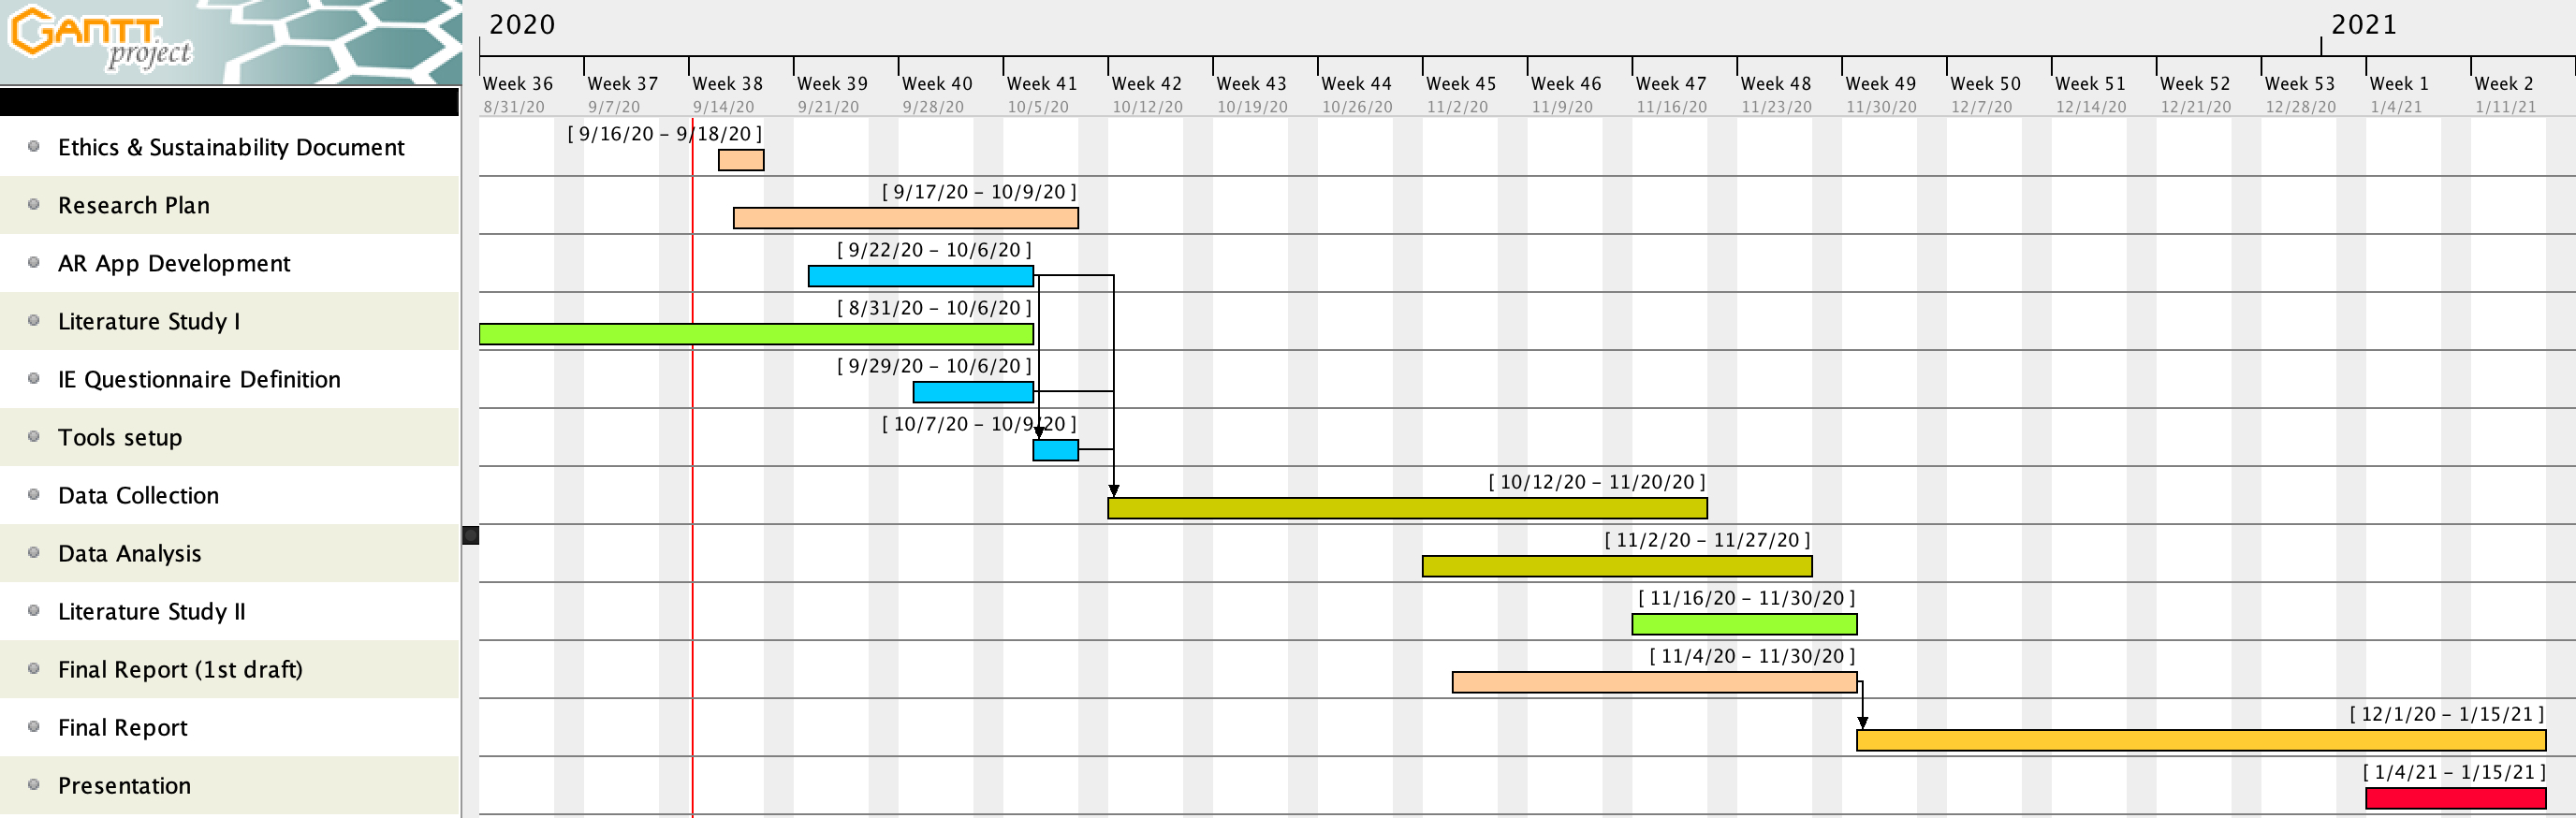
\includegraphics[width=\textwidth]{imgs/project_milestones}

%\todo[inline]{In this section you can additional information that may be relevant to your reader, but is not an answer to any of the above points. Note that the Appendix or Appendices are Optional.}

%The total word count is XXX , with XXX words excluding title, authors, milestone/schedule, references, and words in this sentence, i.e., it is a word count from “Allocation of responsibilities” to end of “Method” section.
%\todo[inline]{The value XXX does not include the instructions and the project plan should be handed in without instructions.}



\section{Acronyms}
\renewcommand{\glossarysection}[2][]{} %% skip the title
\printglossary[type=\acronymtype,nonumberlist]
\clearpage
\end{document}
